
\documentclass[conference]{IEEEtran}
% *** GRAPHICS RELATED PACKAGES ***
%
\ifCLASSINFOpdf
  % \usepackage[pdftex]{graphicx}
  % declare the path(s) where your graphic files are
  % \graphicspath{{../pdf/}{../jpeg/}}
  % and their extensions so you won't have to specify these with
  % every instance of \includegraphics
  % \DeclareGraphicsExtensions{.pdf,.jpeg,.png}
\else
  % or other class option (dvipsone, dvipdf, if not using dvips). graphicx
  % will default to the driver specified in the system graphics.cfg if no
  % driver is specified.
  % \usepackage[dvips]{graphicx}
  % declare the path(s) where your graphic files are
  % \graphicspath{{../eps/}}
  % and their extensions so you won't have to specify these with
  % every instance of \includegraphics
  % \DeclareGraphicsExtensions{.eps}
\fi
% graphicx was written by David Carlisle and Sebastian Rahtz. It is
% required if you want graphics, photos, etc. graphicx.sty is already
% installed on most LaTeX systems. The latest version and documentation can
% be obtained at: 
% http://www.ctan.org/tex-archive/macros/latex/required/graphics/
% Another good source of documentation is "Using Imported Graphics in
% LaTeX2e" by Keith Reckdahl which can be found as epslatex.ps or
% epslatex.pdf at: http://www.ctan.org/tex-archive/info/
%
% latex, and pdflatex in dvi mode, support graphics in encapsulated
% postscript (.eps) format. pdflatex in pdf mode supports graphics
% in .pdf, .jpeg, .png and .mps (metapost) formats. Users should ensure
% that all non-photo figures use a vector format (.eps, .pdf, .mps) and
% not a bitmapped formats (.jpeg, .png). IEEE frowns on bitmapped formats
% which can result in "jaggedy"/blurry rendering of lines and letters as
% well as large increases in file sizes.
%
% You can find documentation about the pdfTeX application at:
% http://www.tug.org/applications/pdftex





% *** MATH PACKAGES ***
%
%\usepackage[cmex10]{amsmath}
% A popular package from the American Mathematical Society that providesnumbersbankability
% many useful and powerful commands for dealing with mathematics. If using
% it, be sure to load this package with the cmex10 option to ensure that
% only type 1 fonts will utilized at all point sizes. Without this option,
% it is possible that some math symbols, particularly those within
% footnotes, will be rendered in bitmap form which will result in a
% document that can not be IEEE Xplore compliant!
%
% Also, note that the amsmath package sets \interdisplaylinepenalty to 10000
% thus preventing page breaks from occurring within multiline equations. Use:
%\interdisplaylinepenalty=2500
% after loading amsmath to restore such page breaks as IEEEtran.cls normally
% does. amsmath.sty is already installed on most LaTeX systems. The latest
% version and documentation can be obtained at:
% http://www.ctan.org/tex-archive/macros/latex/required/amslatex/math/





% *** SPECIALIZED LIST PACKAGES ***
%
%\usepackage{algorithmic}
% algorithmic.sty was written by Peter Williams and Rogerio Brito.
% This package provides an algorithmic environment fo describing algorithms.
% You can use the algorithmic environment in-text or within a figure
% environment to provide for a floating algorithm. Do NOT use the algorithm
% floating environment provided by algorithm.sty (by the same authors) or
% algorithm2e.sty (by Christophe Fiorio) as IEEE does not use dedicated
% algorithm float types and packages that provide these will not provide
% correct IEEE style captions. The latest version and documentation of
% algorithmic.sty can be obtained at:
% http://www.ctan.org/tex-archive/macros/latex/contrib/algorithms/
% There is also a support site at:
% http://algorithms.berlios.de/index.html
% Also of interest may be the (relatively newer and more customizable)
% algorithmicx.sty package by Szasz Janos:
% http://www.ctan.org/tex-archive/macros/latex/contrib/algorithmicx/




% *** ALIGNMENT PACKAGES ***
%
%\usepackage{array}
% Frank Mittelbach's and David Carlisle's array.sty patches and improves
% the standard LaTeX2e array and tabular environments to provide better
% appearance and additional user controls. As the default LaTeX2e table
% generation code is lacking to the point of almost being broken with
% respect to the quality of the end results, all users are strongly
% advised to use an enhanced (at the very least that provided by array.sty)
% set of table tools. array.sty is already installed on most systems. The
% latest version and documentation can be obtained at:
% http://www.ctan.org/tex-archive/macros/latex/required/tools/


%\usepackage{mdwmath}
%\usepackage{mdwtab}
% Also highly recommended is Mark Wooding's extremely powerful MDW tools,
% especially mdwmath.sty and mdwtab.sty which are used to format equations
% and tables, respectively. The MDWtools set is already installed on most
% LaTeX systems. The lastest version and documentation is available at:
% http://www.ctan.org/tex-archive/macros/latex/contrib/mdwtools/


% IEEEtran contains the IEEEeqnarray family of commands that can be used to
% generate multiline equations as well as matrices, tables, etc., of high
% quality.


%\usepackage{eqparbox}
% Also of notable interest is Scott Pakin's eqparbox package for creating
% (automatically sized) equal width boxes - aka "natural width parboxes".
% Available at:
% http://www.ctan.org/tex-archive/macros/latex/contrib/eqparbox/





% *** SUBFIGURE PACKAGES ***
%\usepackage[tight,footnotesize]{subfigure}
% subfigure.sty was written by Steven Douglas Cochran. This package makes it
% easy to put subfigures in your figures. e.g., "Figure 1a and 1b". For IEEE
% work, it is a good idea to load it with the tight package option to reduce
% the amount of white space around the subfigures. subfigure.sty is already
% installed on most LaTeX systems. The latest version and documentation can
% be obtained at:
% http://www.ctan.org/tex-archive/obsolete/macros/latex/contrib/subfigure/
% subfigure.sty has been superceeded by subfig.sty.



%\usepackage[caption=false]{caption}
%\usepackage[font=footnotesize]{subfig}
% subfig.sty, also written by Steven Douglas Cochran, is the modern
% replacement for subfigure.sty. However, subfig.sty requires and
% automatically loads Axel Sommerfeldt's caption.sty which will override
% IEEEtran.cls handling of captions and this will result in nonIEEE style
% figure/table captions. To prevent this problem, be sure and preload
% caption.sty with its "caption=false" package option. This is will preserve
% IEEEtran.cls handing of captions. Version 1.3 (2005/06/28) and later 
% (recommended due to many improvements over 1.2) of subfig.sty supports
% the caption=false option directly:
%\usepackage[caption=false,font=footnotesize]{subfig}
%
% The latest version and documentation can be obtained at:
% http://www.ctan.org/tex-archive/macros/latex/contrib/subfig/
% The latest version and documentation of caption.sty can be obtained at:
% http://www.ctan.org/tex-archive/macros/latex/contrib/caption/




% *** FLOAT PACKAGES ***
%
%\usepackage{fixltx2e}
% fixltx2e, the successor to the earlier fix2col.sty, was written by
% Frank Mittelbach and David Carlisle. This package corrects a few problems
% in the LaTeX2e kernel, the most notable of which is that in current
% LaTeX2e releases, the ordering of single and double column floats is not
% guaranteed to be preserved. Thus, an unpatched LaTeX2e can allow a
% single column figure to be placed prior to an earlier double column
% figure. The latest version and documentation can be found at:
% http://www.ctan.org/tex-archive/macros/latex/base/



%\usepackage{stfloats}
% stfloats.sty was written by Sigitas Tolusis. This package gives LaTeX2e
% the ability to do double column floats at the bottom of the page as well
% as the top. (e.g., "\begin{figure*}[!b]" is not normally possible in
% LaTeX2e). It also provides a command:
%\fnbelowfloat
% to enable the placement of footnotes below bottom floats (the standard
% LaTeX2e kernel puts them above bottom floats). This is an invasive package
% which rewrites many portions of the LaTeX2e float routines. It may not work
% with other packages that modify the LaTeX2e float routines. The latest
% version and documentation can be obtained at:
% http://www.ctan.org/tex-archive/macros/latex/contrib/sttools/
% Documentation is contained in the stfloats.sty comments as well as in the
% presfull.pdf file. Do not use the stfloats baselinefloat ability as IEEE
% does not allow \baselineskip to stretch. Authors submitting work to the
% IEEE should note that IEEE rarely uses double column equations and
% that authors should try to avoid such use. Do not be tempted to use the
% cuted.sty or midfloat.sty packages (also by Sigitas Tolusis) as IEEE does
% not format its papers in such ways.





% *** PDF, URL AND HYPERLINK PACKAGES ***
%
%\usepackage{url}
% url.sty was written by Donald Arseneau. It provides better support for
% handling and breaking URLs. url.sty is already installed on most LaTeX
% systems. The latest version can be obtained at:
% http://www.ctan.org/tex-archive/macros/latex/contrib/misc/
% Read the url.sty source comments for usage information. Basically,
% \url{my_url_here}.
\usepackage{graphicx}
\usepackage{xcolor}
\usepackage{varwidth}
\newcommand{\dofocus}[1]{\textcolor{red}{#1}}



% *** Do not adjust lengths that control margins, column widths, etc. ***
% *** Do not use packages that alter fonts (such as pslatex).         ***
% There should be no need to do such things with IEEEtran.cls V1.6 and later.
% (Unless specifically asked to do so by the journal or conference you plan
% to submit to, of course. )


% correct bad hyphenation here
\pagenumbering{roman}
\hyphenation{op-tical net-works semi-conduc-tor}



\begin{document}
%
% paper title
% can use linebreaks \\ within to get better formatting as desired
\title{Forecasting Hollywood:\\ Can Movie Revenues Be Predicted?}


% author names and affiliations
% use a multiple column layout for up to three different
% affiliations
\author{\IEEEauthorblockN{Muntasir Chowdhury}
\IEEEauthorblockA{School of Computer Science\\
McGill University\\
260558036\\
Email: muntasir.chodhury@mail.mcgill.ca}
\and
\IEEEauthorblockN{Kashif Javed}
\IEEEauthorblockA{School of Computer Science\\
McGill University\\
260535684\\
Email: kashif.javed@mail.mcgill.ca}
\and
\IEEEauthorblockN{Faiz Khan}
\IEEEauthorblockA{School of Computer Science\\
McGill University\\
260435930\\
Email: faiz.khan@mail.mcgill.ca}}

% conference papers do not typically use \thanks and this command
% is locked out in conference mode. If really needed, such as for
% the acknowledgment of grants, issue a \IEEEoverridecommandlockouts
% after \documentclass

% for over three affiliations, or if they all won't fit within the width
% of the page, use this alternative format:
% 
%\author{\IEEEauthorblockN{Michael Shell\IEEEauthorrefmark{1},
%Homer Simpson\IEEEauthorrefmark{2},
%James Kirk\IEEEauthorrefmark{3}, 
%Montgomery Scott\IEEEauthorrefmark{3} and
%Eldon Tyrell\IEEEauthorrefmark{4}}
%\IEEEauthorblockA{\IEEEauthorrefmark{1}School of Electrical and Computer Engineering\\
%Georgia Institute of Technology,
%Atlanta, Georgia 30332--0250\\ Email: see http://www.michaelshell.org/contact.html}
%\IEEEauthorblockA{\IEEEauthorrefmark{2}Twentieth Century Fox, Springfield, USA\\
%Email: homer@thesimpsons.com}
%\IEEEauthorblockA{\IEEEauthorrefmark{3}Starfleet Academy, San Francisco, California 96678-2391\\
%Telephone: (800) 555--1212, Fax: (888) 555--1212}
%\IEEEauthorblockA{\IEEEauthorrefmark{4}Tyrell Inc., 123 Replicant Street, Los Angeles, California 90210--4321}}




% use for special paper notices
%\IEEEspecialpapernotice{(Invited Paper)}




% make the title area
\maketitle


%\begin{abstract}
%\boldmath
We explored the potential of predicting movie gross revenues using the average ratings of the main
cast/crew involved, budget size and the season it was released in. We created a data set by parsing and 
combining movie data from The-Numbers and IMDB. We created maps to take the cast and crew to a real value indicative 
of the average rating that they achieved over all their movies. Using this we created regression predictors
that yield the revenue of the movie given our mappings. We tested four different types of 
regression: standard regression, gradient descent, ridge regression and lasso regression. We determined 
an optimal step size for gradient descent as being 0.00001 for 100,000 iterations and a k = 10 number 
of folds for validation. The standard regression had the best performance being able to predict movie budges with nearly 90\% accuracy.

Our code and data is available at :
\begin{itemize}
\item https://github.com/dridon/aml1/
\item https://github.com/dridon/aml1/tree/master/src/data/features 
\end{itemize}
%\end{abstract}
% IEEEtran.cls defaults to using nonbold math in the Abstract.
% This preserves the distinction between vectors and scalars. However,
% if the conference you are submitting to favors bold math in the abstract,
% then you can use LaTeX's standard command \boldmath at the very start
% of the abstract to achieve this. Many IEEE journals/conferences frown on
% math in the abstract anyway.

% no key




% For peer review papers, you can put extra information on the cover
% page as needed:
% \ifCLASSOPTIONpeerreview
% \begin{center} \bfseries EDICS Category: 3-BBND \end{center}
% \fi
%
% For peerreview papers, this IEEEtran command inserts a page break and
% creates the second title. It will be ignored for other modes.
\IEEEpeerreviewmaketitle

\section{Introduction}
\subsection{Problem Description}
Modern day movie budgets are now reaching near the half billion dollar 
mark. Estimates for the budget of James Cameron's Avatar reach up to
\$425,000,000\cite{topmovies}. As movie budgets grow, so do their
required revenue to yield an acceptable profit for the investment size
presenting an interesting problem. It is important to know the potential 
success of a movie in order to evaluate its investment potential. However, 
movies are complex products shaped by various commercial
and artistic constraints, and require the involvement of
a diverse group of people (cast and crew). In addition to these factors 
a movie's success is affected by marketing, public perception 
and critical ratings. This makes predicting the potential 
revenue for a potential movie a challenge. We describe this more formally 
as follows:

 ``\textit{Produce a predictor using some feature set that allows us 
to accurately estimate the gross revenue for a potential movie.}''

In this document we will describe our attempt at tackling this challenge through
several regression models. We apply our feature set constructed from parsing two
major online movie databases.

\section{Related Work}
\subsection{The Numbers Bankability Index}
The "Hollywood Creative Graph" represents films using 
information about 80,000 people from the movie industry 
and attempts to measure each individual's influence 
on that graph by assigning a "bankability" value 
to them \cite{numbersbank}. This "bankability index" 
is essentially aimed at understanding how much an individual 
should be paid for working on a film using box-office data by 
estimating how much value they bring in to the industry each
year. One may be able to generate the potential revenues by using 
this data. However, this index is commercial and their methodology
private.

\subsection{Word Of Mouth}
Dellarocas et al\cite{dellarocas} leveraged data about a film's initial commercial 
performance, marketing campaign, and early public reaction (word of mouth) 
to forecast revenue. They used a data set of 80 movies with reviews
from over 1,000 critics and nearly 35,000 individuals and fit it to a modified Bass equation. 
They divide the movie into two sets, fit on one and test on the other. They saw a remarkable
success with an error of less than 3\%. 

In a similar vein Rui et al.\cite{rui} and Asur et al.\cite{asur} have tried to gauge the 
influence of "online word of mouth" on movie sales by analysing Twitter data. Rui et al
collected 4,000,000 tweets for 63 movies between June 2009 and February 2010. They took in 
to consideration the authors and the number of followers and the intention of the tweets.
However, they do no cross validation or estimation of true error and directly move on 
to inference from their fit.

Asur et al. used 24 movies with 2.89 million tweets and 1.2 million users. Their fit 
had an R\textsuperscript{2} value of 0.973. However, they also provide no measure
of true error. 

In all cases of \textit{Word Of Mouth}, their methodology is restricted to released
or soon-to-be released movies (otherwise no reviews or tweets will be present) and 
can not be used for movies being considered, planned or in production. Granted that their 
data sets are large, none of the above considered movies greater than 80 in number. This is 
expected because the data collection tasks would be enormous and Twitter data is not available for 
a large number of movies that pre-date the service. Nonetheless, considering that there
is a large range of movies, testing over a small set raises concerns that the fits only 
performed well in local regions.

\subsection{Neural Networks}
Zhang et al\cite{zhang} employ a BP neural-network to predict revenues. They bin
movies in to 6 ordered-categories for classification targets. 
Each representing a different ranges of movie revenues. They
had a maximum of 40 movies per category. Several variables were trained,
some examples being nationality, advertising, content and showing time. They used 
6-fold cross validation and were able to classify a movie correctly with 68.1\%
accuracy and within one class difference with 97.1\% accuracy. 

Their data is also limited by the number of movies they use to train. Also,
their results represent the Chinese market and includes a mixture of Hollywood
and Chinese movies. This data may not be fully reflective of Hollywood earnings. 

\subsection{Other}
Dellarocas \cite{dellarocas} describes the forecasting of motion picture 
revenues to be discernable in to two approaches. The first using 
econometric factors that predict motion picture revenues such 
as The Numbers bankability index. The second using factors that 
influence an individual's decision to watch a movie such as the 
Word Of Mouth approaches. There has been a large amount of work done 
in the prediction of movie revenues and a comprehensive review is out
of the scope for this document. We refer interested readers to \cite{litman-kohl},
\cite{el-el}, \cite{sawhey} and \cite{sochay}.

Most of these approaches use budget and revenue of a film as items in the 
dataset, none factor in the historical critical and audience ratings 
from aggregate movie siteThis suggests our space is linear when trying to predict revenue. 

\section{Dataset Description}
The data set we use to train should be viewed in two parts. The first is the raw data set that 
is generated from mining, parsing, filtering and concatenation that is discussed further
below. The second is the formatted movie set along the actors, directors, producers and screenwriter dictionaries. 

The formatted movie set contains a data point for each movie in the raw set. For each movie we present a boolean 
indicating if they were released during a "hot season". We also present a measure of ratings
by critics and audiences for the directors, producers, screen writers and main actors of the movie. 
Lastly, we have the budget of the movie and the target value, gross revenue for a movie. The dictionaries for 
the cast and crew show their average ratings over all their movies and are used for prediction.

See the appendix for more details.

\section{Methods}
Our methodology is described in three main steps. First, we mine our data from 
two major movie sites and filter it. Then we apply four different regression algorithms 
with cross validation to get initial estimates on errors. Then we apply a set of experiments 
varying parameters in order to draw insights from our data.

\subsection{Libraries}
\begin{table}[h]
\caption{Python Libraries Used In Study}
\label{table:pylibs}
\begin{tabular}{l|l}
Library          & Usage \\
\hline
\\
Beautiful Soup 4\cite{beautifulsoup} & parsing HTML pages \\
unicodecsv\cite{unicodecsv}       & drop-in replacement for csv with unicode support \\
lxml\cite{lxml}             & xml parser for poorly formatted pages \\
numpy\cite{numpy}           & matrix operations\\
scipy\cite{scipy}            & extended operations such as geometric mean \\
scikit-learn\cite{scikit-learn}     & implementations of ridge and lasso regression \\ 
\end{tabular}
\end{table}

A number of libraries were used in our implementations. We describe them briefly in Table \ref{table:pylibs}. 

\subsection{Data Collection}
We extracted our data from two major movie sites: The Numbers \cite{thenumbers} and IMDB\cite{imdb}.
The first is a collection of movie information with budget, revenue, cast, crew with all entries indexed. However, for a large number of movies the information is incomplete. The second one is a large site and community with extensive data but it has no simple movie index to parse data from. A crucial element of our raw data is taken from a third movie aggregation site called Rotten Tomatoes. Instead of parsing the relevant data from the site itself we collected it from The Numbers site.

We first used The Numbers to extract a list of movies, \~20,000 entries, and 
filter the ones that have values for Budgets, Release Dates and 
Revenues, Critic Label/Rating and Audience Label/Rating
(both ratings are from Rotten Tomatoes\cite{rtomato}). 
This gives us around 4,000 movies. We then use the movie names 
collected from The Numbers to search on IMDB for the main cast 
and crew of the movie alongside the IMDB audience rating. We then 
take the union of all the movies with data points for all the 
columns from The Numbers with the IMDB data to get our raw
feature set. This raw set has a size of \~3,300 movies.

\subsection{Feature Selection}
Release Dates and Cast/Crew names are poor features for only 
3,300 examples. Considering there are thousands of individuals amongst
all considered people, we would end up having to estimate 
thousands of values with very little data if we go with something 
along the lines of Naive Bayes. 

We thus create a rating function for all personnel involved in a movie. 
For each director, producer, screen writer and actor, we create a mapping
for the person to the geometric mean of the ratings of all the movies that they 
had significant involvement with. Then for every movie we take the set of actors
and take the average of the mean ratings for all actors involved in the movie. This
gives us a measure on the rating of the movie for the set of actors involved. We 
repeat this for the directors, producers and screenwriters of the movie. 

We produce a rating per person for the "Critical" rating from Rotten Tomatoes, the "Audience" 
rating from Rotten Tomatoes and the IMDB Rating. Thus, we have, for each movie, 
3 measures for each: the set of directors, set of actors, set of producers and 
the set of screen writers giving us a total of 12 features. 

We then label the summer months between May and August (inclusive) and the 
holiday season of November and December together to be the 6 months giving
us the "hot season". We then convert the Release Dates to indicate a 1 
for being released during the hot season and 0 otherwise. 

Lastly, since movie budgets and revenues can range from thousands
to hundreds of millions, we take the base 10 logarithms of each to
compress the possible inputs and outputs. For some cases we had a 
few cases (less than 50) where there were \$0 revenues. For these we used a 
revenue of \$1, a small increment considering the rest are many orders
of magnitudes higher, that helps smoothen out the transformation.

We are thus left with 14 features and a target value all in real numbers making 
regression an optimal choice.

\subsection{Algorithms}
We investigated four regression algorithms in our study: 
Standard Linear Regression, Gradient Descent, Ridge Regression and 
Lasso Regression.

\subsubsection{Standard Linear Regression}
We apply the standard form of linear regression with the least-squared error 
in closed form. We initially investigate a 10-fold validation and present the results
for each of the test sets along with the mean squared error. We then 
range k from 10 to 33, bounding the size of the test set below by atleast 100 movies, 
and present the mean squared error for each k. 

\subsubsection{Gradient Descent}
We apply gradient descent using the least squared error. We first vary alpha and 
use cross validation error to obtain an estimate for an optimal alpha with 100,000 iterations.
The alphas vary from 10\textsuperscript{-5} to 10\textsuperscript{-8} with one order of magnitude increments. 
We then use that alpha to determine an optimal iteration. After that we use the optimal alpha
and iteration values in the general analysis of our predictability. We vary iterations from
10\textsuperscript{1} to 10\textsuperscript{5} increments, simply because execution time becomes unfeasible.
We also use these values to train the predictor for the full feature set. We use 10,000 iterations 
for varying the k parameter because the processing time was not available. 

\subsubsection{Ridge and Lasso}
We apply the ridge and lasso from the scikit-learn library. We repeat the experiments
done for standard regression on ridge and lasso and present their results.

\subsubsection{Cross Validation}
In order to test on a prediction we need a method to map a given set of actors, directors or producers to
their average rating. We cannot create this prior to cross validation because we will be using the test set 
and potentially corrupting our data. Thus we have to generate these mappings from an individual to rating 
each time for during each fold in cross validation and essentially regenerate the entire feature set. 
In the case that an actor, director, producer or screen writer is not present in a mapping, we simply assign 
them a 50\% rating for Rotten Tomatoes and 5.0 for IMDB. That is we do not assume any information for missing cases.

The cross validation scheme is done as follows: 
\begin{enumerate}
\item The raw feature set, R, is loaded as a list of movie features for each movie
\item The movies are shuffled around in R to get R' 
\item R' is then divided in to k folds 
\item For each fold f in the k fold we merge all but fold f in to f' 
\item We train on f', to get predictor P and generate mappings from an individual to their average rating call M 
\item We use M to convert the f fold into input parameters and test the predictions against the actual values 
\item Then we take the mean of all the errors from the k runs to estimate the true error 
\end{enumerate}

\section{Results}

We present the results of our experiments in this section and expand 
on them in the next. It should be noted that all errors are mean square errors of
the log10 of the revenue. This means that a mean square error of 
one means that there is a one order of magnitude difference between the true estimate 
of revenue and our predicted value. 

\begin{center}

%Error chart for Gradient Descent with varying alpha
\begin{figure}[ht!]
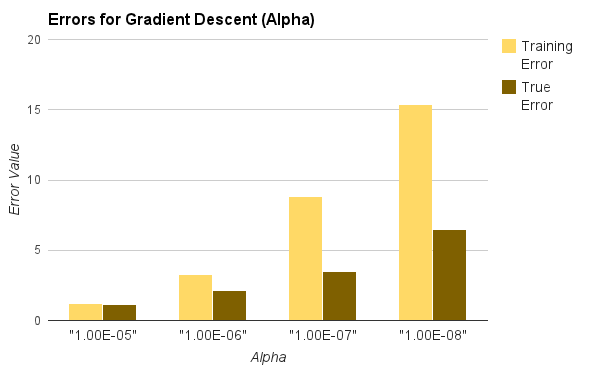
\includegraphics[width=90mm]{gdAlpha.png}
\caption{}\label{fig:alphahist}
\end{figure}

%Error chart for Gradient Descent with varying number of iterations
\begin{figure}[ht!]
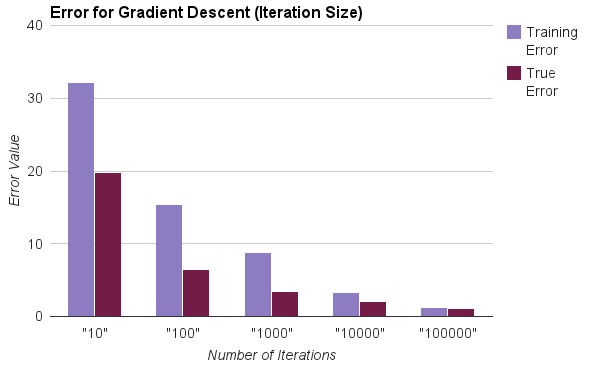
\includegraphics[width=90mm]{gdIteration.png}
\caption{}\label{fig:iterhist}
\end{figure}
\end{center}

We first present the results for the determination of an optimal alpha for gradient descent in Figure \ref{fig:alphahist}. 
The training error and true error estimate are shown with the variation of the step size. Similar results are in Figure \ref{fig:iterhist} for the variation of the iteration size for gradient descent. 

We determine the optimal value for alpha to be around 0.0001 with an iteration count of 100,000. We then use this 
to estimate gradient descent weights along with the other regressions under consideration. Table \ref{table:regweights} shows
the prediction weights using the entire data set for training. It should be noted, the weights in the cross validation
would be slightly different. 

\begin{table}[h]
\caption{Regression Weights for different predictors}
\label{table:regweights}
\begin{tabular}{lllll}
                                 &SR       & GD & Ridge  & Lasso\\
Hot Season                       & 0.015        & 0.634            & 0.016  & 0.0000  \\
Budget                           & 1.081        & 0.393            & 1.080  & 0.0000  \\
Director RT Critical Average     & -0.005       & -0.006           & -0.005 & 0.0000  \\
Director RT Public Average       & 0.006        & 0.004            & 0.006  & 0.0032  \\
Director IMDB Average            & 0.043        & 0.147            & 0.043  & 0.0000  \\
Producer RT Critical Average     & -0.004       & -0.008           & -0.004 & -0.0074 \\
Producer RT Public Average       & 0.005        & 0.004            & 0.005  & 0.0010  \\
Producer IMDB Average            & 0.129        & 0.184            & 0.128  & 0.0000  \\
Screenwriter RT Critical Average & 0.003        & -0.001           & 0.003  & 0.0000  \\
Screenwriter RT Public Average   & 0.010        & 0.002            & 0.010  & 0.0031  \\
Screenwriter IMDB Average        & -0.155       & 0.103            & -0.154 & 0.0000  \\
Actors RT Critical Average       & 0.003        & -0.009           & 0.003  & 0.0000  \\
Actors RT Public Average         & -0.002       & -0.006           & -0.002 & 0.0000  \\
Actors IMDB Average              & -0.145       & -0.102           & -0.145 & 0.0003  \\
Intercept                        & -0.178       & -0.132           & -0.178 & 0.0003 
\end{tabular}
\\
SR and GD stand for standard regression and gradient descent, respectively.
\end{table}

The error for each k for each regression is shown in Figure \ref{fig:foldgraph}. This figure shows how
the error changes as we increase the value of k. Standard and Ridge regression were essentially the same 
thus their curves overlap on the figure. Noticing the k value does 
not seem to affect the error estimate after k = 10, we simply use it as our cross validation
number. The results for true and training error for 10-fold validation are then presented in 
the histogram in Figure \ref{fig:errorhist}.

\begin{center}

%Error chart for all methods with varying fold size
\begin{figure}[ht!]
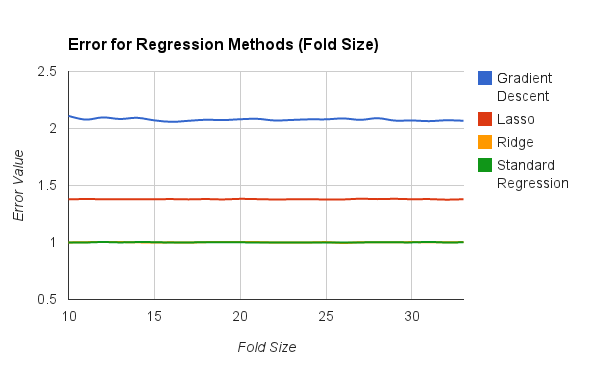
\includegraphics[width=90mm]{errFoldSize.png}
\caption{}\label{fig:foldgraph}
\end{figure}

%Error chart for all methods. Has 10-fold cross validation
\begin{figure}[ht!]
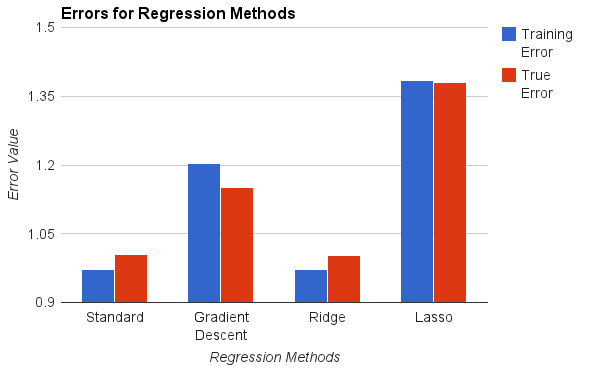
\includegraphics[width=90mm]{errorHistogramWith10fold.png}
\caption{}\label{fig:errorhist}
\end{figure}
\section{Discussion}
\end{center}
Although our results seem to show that our predictor is fairly 
successful, there are some cases such as Gradient Descent that 
are alarming and raise questions. To discuss these further we now 
proceed to analyze the results presented in the previous section. 

\subsection{Analysis}
In our analysis for gradient descent from Figure \ref{fig:alphahist}, we notice that for an iteration
count of 100,000 the error increases after 0.00001. This means 
that more iterations are needed to improve the error after this step size. 
However, iteration sizes of 100,000 and higher did not terminate in a feasible 
amount of time for us to perform experiments on, thus 0.00001 was optimal for
our needs.

The iteration count however showed the opposite trend in Figure \ref{fig:iterhist}. 
The higher the iteration count the better the error estimate proved to be. However, again,
our resources were limited and we chose 100,000 for our experiments apart from the 
variation of the size of folds on which we used 10,000 as our iteration size. 

Gradient descent proved problematic because it constantly showed a better test error 
over a training error in Figure \ref{fig:alphahist}, Figure~\ref{fig:iterhist} and Figure \ref{fig:errorhist}. 
We were not able to isolate the reason as to why this seems to be the case in only this 
regression. The data is always randomly shuffled before a validation and this phenomenon repeated 
multiple times thus we don't believe that the test error is performing better simply because 
of a local distribution. Other predictors did not show this issue thus we are still able to draw
important insights from them. 

The weights shown in Table \ref{table:regweights} vary significantly depending on the regression task. Standard and 
Ridge Regression both produce the same results. Figure \ref{fig:errorhist} also shows these to be the best
estimators of our data with error values of around 1, which results in around a 90\% success rate since its 
a log10 of the revenue. As one would expect the highest weight seems to be on the budget. Taking in to account the IMDB ratings being out of 10 and RottenTomato ratings are out of 100, it seems that the IMDB ratings still reflect
the revenue a bit more strongly then the RottenTomato ratings. Gradient Descent on the other hand places 
the most weight on the season the movie is released on. Lasso seems to suggest that the majority of the 
weights are small enough to be ignored. 

It is also reflected that our k-fold validation did not change with the k parameter as shown in Figure \ref{fig:foldgraph}.
This could be due to the size of our small data set. A fold size of k = 10 will produce a test set of size around 330
and k = 33 will produce a size around 100. This means the training set was, the same for the most part. We were unable to explore smaller sizes due to time constraints. 

Overall the best performer is standard regression with an error of around 1 and the worst performer is Lasso with an error of around 1.4. Thus our best predictor shows an accuracy around 90\%. Since our results seem to be successful over the majority of our experiments we also feel that the movie prediction space is linear in nature. 

\subsection{Applications }
The most immediate application would be to implement the predictor as a tool that allows an user to choose the different parameters for a movie (budget, actors, directors) and get an estimate of the revenue. Training the tool
on a larger database consisting of a more complete list of movies such as the entire IMDB website. Using this
financial decisions may be made that include the initiation of a movie production, cancellation or budget change. 

Even if a studio does not use the tool for the initial planning of a film it might turn out useful when it's trying to determine the final parameters of the film. For example, a scenario where all the cast and crew of a film have been hired and the lead actor still needs to be chosen. The studio may be able to generate a list of likely candidates using this predictor to determine the most optimal choices. The tool would go through the entire database of actors and list the ones whose involvement would result in the highest revenue.

\subsection{Future Perspectives}
Our initial data set of 20,000 films had to be drastically reduced when we aimed to discard incomplete entries. As a first
step, a larger dataset of complete data points would give more insights about the model. More ratings for existing entries 
could be added from another major aggregate site called Metacritic. This could lead to more accurate results or give us an idea
of which site's rating model is better.

Finally, another interesting prediction question would be to calculate a movie's potential critical rating or reception. Tweaking parameters
for high critical success could be one application. But a more interesting one would be to have a model which tries to optimize both critical
and commercial success simultaneously.

\section{Conclusion}
We explored the potential of predicting movie gross revenues using the average ratings of the main
cast/crew involved, budget size and the season it was released in. We tested four different types of 
regression: standard regression, gradient descent, ridge regression and lasso regression. We determined 
an optimal step size for gradient descent as being 0.00001 for 100,000 iterations and a k = 10 number 
of folds for validation. The largest discrepancy was with gradient descent that consistently showed 
a higher training error as compared to a test error. However, none of the other regressions presented this issue and results showed that standard regression had the best performance, being able to predict movie budges with nearly 90\% accuracy.

\section*{Statement Of Original Work}

We hereby state that all the work presented in this report is that of the authors.


\begin{thebibliography}{1}
\bibitem{topmovies}
"Movie Budget and Financial Performance Records" (The-Numbers)  [online], http://www.the-numbers.com/movie/budgets/ (Accessed:15 September 2014)

\bibitem{numbersbank}
"The Numbers Bankability Index" (The-Numbers) [online], http://www.the-numbers.com/bankability/ (Accessed:15 September 2014)

\bibitem{thenumbers}
"The-Numbers" (The-Numbers) [online], http://www.the-numbers.com/ (Accessed: 15 September 2014)

\bibitem{dellarocas}
C. Dellarocas, N. Awad and X. Zhang, 2004, "Exploring the Value of Online Reviews to Organizations: Implications for Revenue Forecasting and Planning", ICIS 2004 Proceedings

\bibitem{rui}
H. Rui, Y. Liu and A. Whinston, 2013, "Whose and what chatter matters? The effect of tweets on movie sales", Decision Support Systems 55.4 (2013): 863-870

\bibitem{asur}
S. Asur and B. Huberman, 2010, "Predicting the Future with Social Media", Web Intelligence and Intelligent Agent Technology (WI-IAT), 2010 IEEE/WIC/ACM International Conference on. Vol. 1, pp 492 - 499

\bibitem{zhang}
L Zhang, J Luo and S Yang, 2009, "Forecasting box office revenue of movies with BP neural network." Expert Systems with Applications 36.3 (2009): 6580-6587

\bibitem{litman-kohl}
B. Litman and L. Kohl, 1989, "Predicting financial success of motion pictures: The'80s experience." Journal of Media Economics 2.2 (1989), pp 35-50

\bibitem{el-el}
M Sawhney and J. Eliashberg, 2002, "The drivers of motion picture performance: the need to consider dynamics, endogeneity and simultaneity." proceedings of the Business and Economic Scholars Workshop in Motion Picture Industry Studies. Florida Atlantic University

\bibitem{sawhey}
M Sawhney and J. Eliashberg, 1996, “A Parsimonious Model
for Forecasting Gross Box-Office Revenues of Motion Pictures,” Marketing Science 15.2, pp 113-131.

\bibitem{sochay}
S. Sochay, "Predicting the performance of motion pictures." Journal of Media Economics 7.4 (1994), pp 1-20

\bibitem{zufryden}
F. Zufryden, 1996, "Linking advertising to box office performance of new film releases: A marketing planning model." Journal of Advertising Research 36 (1996), pp 29-42

\bibitem{imdb}
"IMDb - Movies, TV and Celebrities" (IMDB) [online], http://www.imdb.com/ (Accessed: 15 September 2014)

\bibitem{rtomato}
"Rotten Tomatoes" (Rotten Tomatoes) [online], http://www.rottentomatoes.com/ (Accessed: 15 September 2014)

\bibitem{beautifulsoup}
"Beautiful Soup" (Crummy) [online], http://www.crummy.com/software/BeautifulSoup/ (Accessed: 15 September 2014)

\bibitem{unicodecsv}
"unicodecsv 0.9.4" (Python) [online], https://pypi.python.org/pypi/unicodecsv/0.9.4 (Accessed: 15 September 2014)

\bibitem{lxml}
"lxml - Processing XML and HTML with Python" (lxml) [online], http://lxml.de/ (Accessed: 15 September 2014)

\bibitem{numpy}
"NumPy" (NumPy) [online], http://www.numpy.org/ (Accessed: 15 September 2014)

\bibitem{scipy}
"SciPy" (SciPy) [online], http://www.scipy.org/ (Accessed: 15 September 2014)

\bibitem{scikit-learn}
"scikit-learn: machine learning in Python" (scikit-learn) [online], http://scikit-learn.org/stable/ (Accessed: 15 September 2014)

\end{thebibliography}

\newpage
\section{Appendix}

\subsection{Data Dictionary}

Initially we downloaded the indexed movie pages from The Numbers. After filtering out the entries that were missing too many relevant fields we queried the IMDB search engine for the remaining movies. We downloaded these pages and used the information there to add the IMDB score and fill in whatever fields were empty in the remaining movie list. The "full\_raw\_features.csv" contains the data parsed from The Numbers movie pages and the IMDB page. Each entry is a movie and contains the following information:

Movie Name, Release Date, Genre, Budget, Gross, RT Critic Label, RT Critic Rating, RT Audience Label, RT Audience Rating, IMDB Rating, Directors, Producers, Sreenwriters, and Actors.
\\*\textbf{RT Critic Rating} - This is the "Critical Rating" given to a movie on Rotten Tomatoes. Rotten Tomatoes aggregates movie reviews from major critics and publications and gives them a quantitative value. It then takes the average of those values to produce the Critical Rating.
\\*\textbf{RT Audience Rating} - This is the average of the ratings given to a movie by registered users on the Rotten Tomatoes website.
\\*\textbf{RT Critic Label and RT Audience Label} - We do not end up using these in the final feature set. 
\\*\textbf{IMDB Rating} - This is the average of the ratings given to a movie by registered users on the IMDB website.
\\*\textbf{Director} - The name of the director(s) of the movie.
\\*\textbf{Producers} - Names of the studio that produced the movie.
\\*\textbf{Screenwriters} - Names of all the screenwriters of the movie.
\\*\textbf{Actors} - The first 3 names from the actor lists on The Numbers and the IMDB movie pages. These lists are in order of importance of the actor in the movie.\\
From this file we calculated the three kinds of ratings for every unique director, producer, screenwriter and actor. These are listed in four separate data files for each type of the four mentioned types.\\*

\textbf{Person's RTC Mean} - The average of the Critical Ratings for all the movies the person is listed in. If a person has been in the role of both a director and an actor then her values for each role are independent and mutually exclusive.\\*
\textbf{Person's RTA Mean} - The average of the Audience Ratings for all the movies the person is listed in.\\*
\textbf{Person's IMDB Mean} - The average of the Critical Ratings for all the movies the person is listed in.\\*

From these we form our final feature set, a version of which is outputted in "feature.csv". The format is outlined below.

\begin{table}[h]
\caption{Feature Set}
\label{table:datadict}
\begin{tabular}{l|l}
Feature          & Description \\
\hline
\\
Hot Season & This is 0 or 1 depending on the\\* & release date\\ 
Budget & The log of the movie's budget \\* & in dollars \\
Director RT Critical Average & Average of the RTC Mean for all\\* & directors involved\\
Director RT Public Average & Average of the RTA Mean for all\\* & directors involved\\
Director IMDB Average & Average of the IMDB Mean for all\\* & directors involved\\
Producer RT Critical Average & Average of the RTC Mean for all\\* & studios involved\\
Producer RT Public Average & Average of the RTA Mean for \\* & all studios involved\\
Producer IMDB Average &  Average of the IMDB Mean for \\* & all studios involved\\
Screenwriter RT Critical Average & Average of the RTC Mean for all \\* & screenwriters involved\\
Screenwriter RT Public Average & Average of the RTA Mean for all \\* & screenwriters involved\\
Screenwriter IMDB Average & Average of the IMDB mean for all \\* & screenwriters involved (DT)\\ 
Actors RT Critical Average & Average of the RTC Mean for all \\* & actors involved\\
Actors RT Public Average  & Average of the RTA Mean for all\\* & actors involved\\
Actors IMDB Average &  Average of the IMDB Mean for all\\* & actors involved\\     &\\ 
\end{tabular}
\end{table}

\begin{table}[h]
\caption{Output Set}
\label{table:datadict}
\begin{tabular}{l|l}
Output          & Description \\
\hline
\\
Gross & The log of the movie's revenue in dollars\\
\end{tabular}
\end{table}

The \textbf{Hot Season} is set to 1 if a film was released in the months of either May to August OR November-December. It is set to 0 otherwise. May to August is generally referred to as the summer blockbuster season when movie revenues are higher. This is due to schools being closed during that time and release of higher budget movies being concentrated around that period. November and December coincide with the holiday season and sees the release of award-season movies and critical favorites.

A crucial point to note is that this feature set is derived from the training data we have. If we change the number of data points for the training data then the values in the ratings file for director, producer, screenwriter and actor will change. As a result so will the average people ratings for movies in "full\_raw\_features.csv".


% that's all folks
\end{document}

